\documentclass[11pt]{article}
\usepackage[utf8]{inputenc}
\usepackage[T1]{fontenc}
\usepackage{grffile}
\usepackage{longtable}
\usepackage{wrapfig}
\usepackage{rotating}
\usepackage[normalem]{ulem}
\usepackage{amsmath}
\usepackage{textcomp}
\usepackage{amssymb}
\usepackage{capt-of}
\usepackage{hyperref}
\hypersetup{colorlinks=true, linkcolor=magenta}
\setlength{\parindent}{0in}
\usepackage[margin=1in]{geometry}
\usepackage[spanish]{babel}
\usepackage{mathtools}
\usepackage{palatino}
\usepackage{fancyhdr}
\usepackage{sectsty}
\usepackage{engord}
\usepackage{parskip}
\usepackage{minted}
\usepackage{cite}
\usepackage{graphicx}
\usepackage{subcaption}
\usepackage{setspace}
\usepackage[compact]{titlesec}
\usepackage[center]{caption}
\usepackage{placeins}
\usepackage{color}
\usepackage{amsmath}
\usepackage{varwidth}
\usepackage{bm}
\usepackage{todonotes}
\usepackage{pdfpages}
% \titlespacing*{\subsection}{0pt}{5.5ex}{3.3ex}
% \titlespacing*{\section}{0pt}{5.5ex}{1ex}
\decimalpoint
\author{Antonio Coín Castro}
\date{\today}
\title{Aprendizaje Profundo para Procesamiento de Señales de Imagen y Vídeo\\\Large{Práctica 1}}
\hypersetup{
 pdfauthor={Antonio Coín Castro},
 pdftitle={},
 pdfkeywords={},
 pdfsubject={},
 pdflang={Spanish}}

\begin{document}

\maketitle

\section{SimpleCNN}

En el primer notebook, \verb|Image_Classification_1.ipynb|, desarrollamos una arquitectura CNN simple para clasificación de imágenes del conjunto MNIST (dígitos manuscritos en escala de grises).

\subsection*{Resumen del dataset}

En \verb|Pytorch| disponemos directamente del dataset \href{https://pytorch.org/vision/stable/datasets.html#mnist}{MNIST} como \textit{built-in}.

\begin{table}[h!]
   \centering
  \begin{tabular}{c|cccc}
    & Alto de imagen & Ancho de imagen & Nº canales de imagen & Nº muestras\\
    \hline
    Entrenamiento & 28 & 28 & 1 & 60000\\
    Validación & 28 & 28 & 1 & 10000\\
  \end{tabular}
\end{table}

\subsection*{Arquitectura de SimpleCNN}

Construimos una red sencilla con dos capas convolucionales con kernels $3\times 3$ y activación ReLu, y dos capas totalmente conectadas. Añadimos una capa \textit{Max-Pooling} $2\times 2$ para realizar \textit{downsampling} y capas \textit{Dropout} para añadir regularización. En resumen, la arquitectura queda como sigue:

\begin{table}[h!]
  \centering
  \begin{tabular}{c|cccc}
    Capa & Output shape & Nº canales output & Nº parámetros entrenables\\
    \hline
    Conv2D & 28\times 28 & 32 & 320\\
    ReLu & 28\times 28 & 32 & 0\\
    Conv2D & 28 \times 28 & 32 & 9248\\
    ReLu & 28\times 28 & 32 & 0\\
    MaxPool2D & 14\times 14 & 32 & 0\\
    Dropout$(0.25)$ & 14\times 14 & 32 & 0\\
    Flatten & 6272\times 1 & 1 & 0\\
    Linear & 128\times 1 & 1 & 802944\\
    ReLu & 128\times 1 & 1 & 0\\
    Dropout$(0.5)$ & 128\times 1 & 1 & 0\\
    Linear & 10\times 1 & 1 & 1290\\
    \hline
    \textit{Nº total de parámetros} & & & {813802}
  \end{tabular}
\end{table}

\subsection*{Curvas de aprendizaje y precisión}

Entrenamos nuestro modelo durante 10 épocas, obteniendo las curvas de entrenamiento y validación de la Figura \ref{fig:1_lc}.

\begin{figure}[h!]
  \centering
  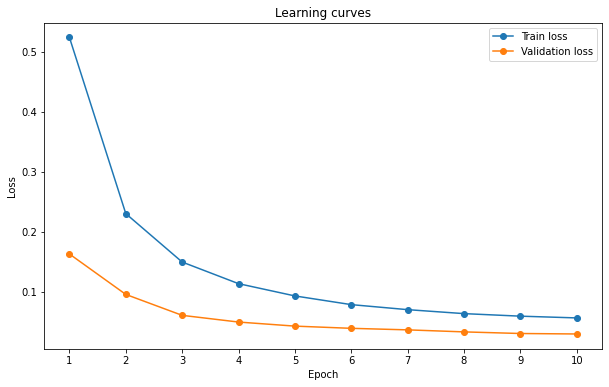
\includegraphics[width=.7\textwidth]{img/1_learning_curves}
  \caption{Curvas de entrenamiento y validación de SimpleCNN en 10 épocas.}
    \label{fig:1_lc}
\end{figure}

Observamos que no se aprecia \textit{overfitting}, ya que la pérdida en validación se mantiene siempre por debajo de la pérdida en entrenamiento, y además ambas curvas van descendiendo conforme aumentan las épocas. Tampoco se aprecian problemas de \textit{underfitting} ó \textit{high-bias}, ya que el modelo sí que está aprendiendo (como hemos dicho, la pérdida va disminuyendo). Esto se debe muy probablemente, además de a la adecuación del modelo a los datos, a la presencia de capas de regularización \textit{Dropout} en entrenamiento (y obviamente su ausencia en validación), que hacen que aumente la capacidad de generalización.

En cuanto a la precisión en validación, obtenemos el siguiente resultado:

\begin{table}[h!]
  \centering
  \begin{tabular}{c|cc}
    & Mejor precisión (validación) & Época con mejor precisión\\
    \hline
    SimpleCNN & $98.98\%$ & 10
  \end{tabular}
\end{table}

Vemos que es un muy buen resultado, con una precisión bastante cercana al $100\%$. Vistas las curvas de aprendizaje, es probable que el modelo siguiera aprendiendo si seguimos entrenando durante más épocas, ya que parece que la pérdida en validación sigue descendiendo y no ha llegado aún al punto óptimo. De hecho, podemos comprobar esta hipótesis continuando con el entrenamiento del modelo durante 10 épocas más. Si lo hacemos, obtenemos la curva completa de aprendizaje de la Figura \ref{fig:1_lc_full}. Efectivamente, conseguimos aumentar la precisión en validación máxima hasta el $99.22\%$, y ya la curva de validación parece haberse estancado e incluso empieza a aumentar ligeramente, por lo que el modelo probablemente ya no se beneficiaría mucho de más épocas de entrenamiento.

\begin{figure}[h!]
  \centering
  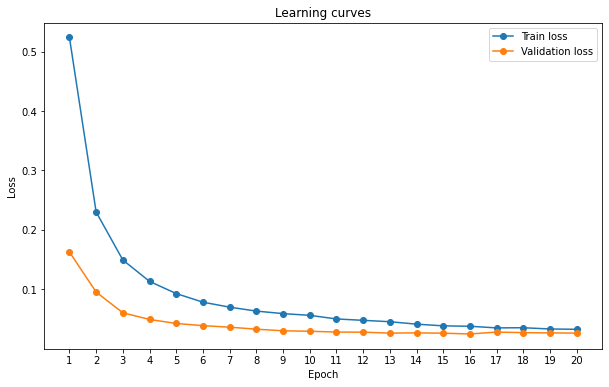
\includegraphics[width=.7\textwidth]{img/1_learning_curves_full}
    \caption{Curvas de entrenamiento y validación de SimpleCNN en 20 épocas.}
    \label{fig:1_lc_full}
\end{figure}

\subsection*{Matriz de confusión}

Otra de las formas de evaluar el modelo es mostrar la matriz de confusión, que mide el número de aciertos y fallos entre las predicciones y los valores reales para todas las etiquetas por separado. En nuestro caso podemos verla para el conjunto de validación en la Figura \ref{fig:1_confusion_matrix}.

\begin{figure}[h!]
  \centering
  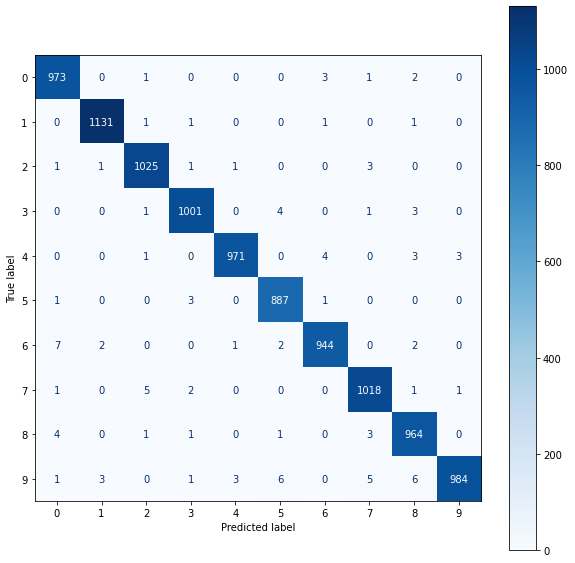
\includegraphics[width=.5\textwidth]{img/1_confusion_matrix}
  \caption{Matriz de confusión en validación para el modelo SimpleCNN tras 10 épocas.}
  \label{fig:1_confusion_matrix}
\end{figure}

Analizando los resultados, vemos que en total cometemos 102 errores (de un total de 10000 predicciones). Los dígitos que más se confunden son el 6 con el 0, con 7 fallos, seguidos del 9 con el 5 y el 8, con 6 fallos en cada caso. Todos ellos son dígitos relativamente fácilmente de confundir por su forma, dependiendo de la persona que los escriba.

\subsection*{Proyecciones t-SNE}

Incluimos a continuación en la Figura \ref{fig:1_tsne} las proyecciones \href{https://scikit-learn.org/stable/modules/generated/sklearn.manifold.TSNE.html}{t-SNE} de la representación de las capas intermedia y final de la red para los datos de validación.

\begin{figure}[h!]
     \centering
     \begin{subfigure}[b]{0.45\textwidth}
         \centering
         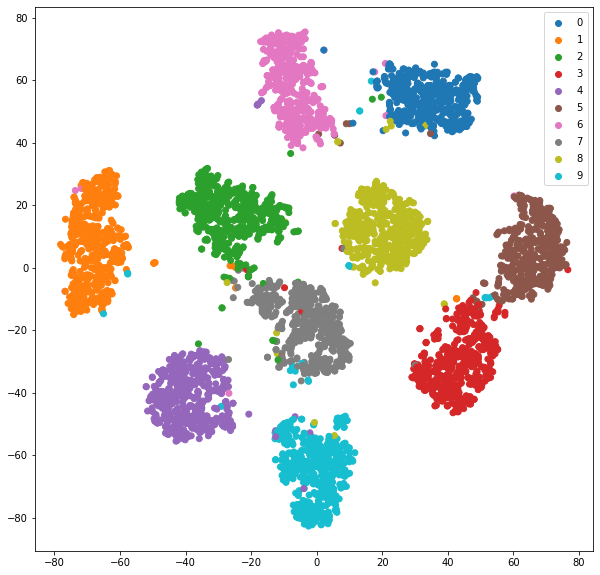
\includegraphics[width=\textwidth]{img/1_tsne_intermediate}
         \caption{Representación intermedia}
     \end{subfigure}
     \hfill
     \begin{subfigure}[b]{0.45\textwidth}
         \centering
         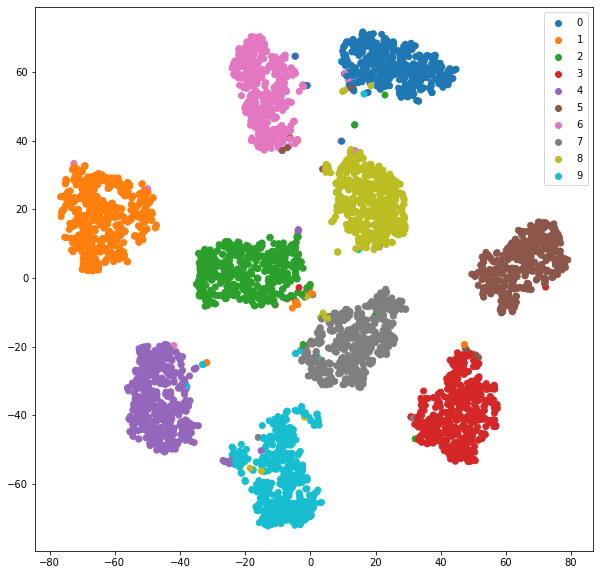
\includegraphics[width=\textwidth]{img/1_tsne_final}
         \caption{Representación final}
     \end{subfigure}
        \caption{Proyecciones t-SNE de las representaciones de SimpleCNN.}
        \label{fig:1_tsne}
\end{figure}

Como vemos, con la representación intermedia ya obtenemos 10 clústers claramente diferenciados, cada uno correspondiente a un dígito distinto. El hecho de que se formen estos grupos tras la proyección en 2D hace pensar que la capacidad discriminativa de la red tras la capa intermedia es suficiente para clasificar con éxito los dígitos. Sin embargo, vemos que se observa cierto solapamiento en algunos clústers (por ejemplo en el 7 y en el 2), y que otros grupos están un poco dispersos (por ejemplo el 1). Si pasamos a la representación final vemos que los clústers están ya más separados y más compactos, lo que sugiere que la clasificación a partir de las características finales será aún mejor\footnote{Aunque tras la representación t-SNE obtengamos clústers diferenciados, esto no garantiza en principio que la clasificación en el espacio original vaya a ser igual de buena, aunque es probable que así sea.}.
\newpage

\section{AlexNet}

En este caso pasamos al conjunto \href{https://pytorch.org/vision/stable/datasets.html#cifar}{CIFAR10}, también disponible en \verb|Pytorch|, que consta en total de 60000 imágenes RGB pertenecientes a diez clases balanceadas. El notebook asociado es \verb|Image_Classification_2.ipynb|.

\subsection*{Arquitectura de AlexNet}

\begin{minted}{python}
class AlexNet(nn.Module):
  def __init__(self, output_dim):
    super(AlexNet, self).__init__()

    self.features = nn.Sequential(
      nn.Conv2d(3, 48, 5, 2, 2),
      nn.MaxPool2d(2),
      nn.ReLU(inplace = True),

      nn.Conv2d(48, 128, 5, 1, 2),
      nn.MaxPool2d(2),
      nn.ReLU(inplace = True),

      nn.Conv2d(128, 192, 3, 1, 1),
      nn.ReLU(inplace = True),
      nn.Conv2d(192, 192, 3, 1, 1),
      nn.ReLU(inplace = True),

      nn.Conv2d(192, 128, 3, 1, 1),
      nn.MaxPool2d(2),
      nn.ReLU(inplace = True)
  )

  self.classifier = nn.Sequential(
      nn.Dropout(0.5),
      nn.Linear(128*2*2, 2048), # final conv layer resolution 2x2
      nn.ReLU(inplace = True),

      nn.Dropout(0.5),
      nn.Linear(2048, 2048),
      nn.ReLU(inplace = True),

      nn.Linear(2048, output_dim)
    )

  def forward(self, x):
      x = self.features(x)
      interm_features = x.view(x.shape[0], -1)
      x = self.classifier(interm_features)
      return x, interm_features
\end{minted}

Podemos ver a continuación el modelo generado a partir del código anterior, donde apreciamos que el número total de parámetros entrenables asciende a $6199498$.
\vspace{1em}
\begin{figure}[h!]
  \centering
  \begin{varwidth}{\linewidth}
\begin{verbatim}
----------------------------------------------------------------
        Layer (type)               Output Shape         Param #
================================================================
            Conv2d-1           [-1, 48, 16, 16]           3,648
         MaxPool2d-2             [-1, 48, 8, 8]               0
              ReLU-3             [-1, 48, 8, 8]               0
            Conv2d-4            [-1, 128, 8, 8]         153,728
         MaxPool2d-5            [-1, 128, 4, 4]               0
              ReLU-6            [-1, 128, 4, 4]               0
            Conv2d-7            [-1, 192, 4, 4]         221,376
              ReLU-8            [-1, 192, 4, 4]               0
            Conv2d-9            [-1, 192, 4, 4]         331,968
             ReLU-10            [-1, 192, 4, 4]               0
           Conv2d-11            [-1, 128, 4, 4]         221,312
        MaxPool2d-12            [-1, 128, 2, 2]               0
             ReLU-13            [-1, 128, 2, 2]               0
          Dropout-14                  [-1, 512]               0
           Linear-15                 [-1, 2048]       1,050,624
             ReLU-16                 [-1, 2048]               0
          Dropout-17                 [-1, 2048]               0
           Linear-18                 [-1, 2048]       4,196,352
             ReLU-19                 [-1, 2048]               0
           Linear-20                   [-1, 10]          20,490
================================================================
Total params: 6,199,498
Trainable params: 6,199,498
Non-trainable params: 0
----------------------------------------------------------------
\end{verbatim}
\end{varwidth}
\end{figure}

\subsection*{Curvas de aprendizaje y precisión}

Si entrenamos el modelo durante 15 épocas, obtenemos las curvas de entrenamiento y validación de la Figura \ref{fig:2_curvas}. Vemos que en un principio el modelo aprende sin caer en \textit{overfitting} (ambas pérdidas van descendiendo casi a la par), pero a partir de aproximadamente la época 10 la pérdida en validación comienza a estancarse y luego a aumentar. Esto nos lleva a la conclusión de que hemos pasado el punto óptimo de \textit{early stopping} y el modelo está empezando a sobreajustar, y que por tanto continuar con más épocas no mejoraría el rendimiento del mismo.

\begin{figure}[h!]
  \centering
  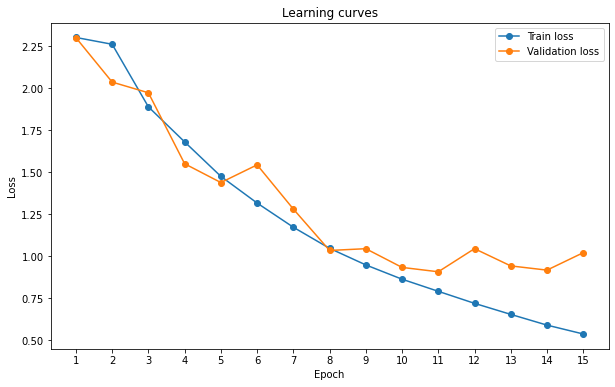
\includegraphics[width=0.7\textwidth]{img/2_learning_curves}
  \caption{Curvas de entrenamiento y validación de AlexNet en 15 épocas.}
  \label{fig:2_curvas}
\end{figure}

Por otra parte, los mejores resultados de precisión en validación son los siguientes:

\begin{table}[h!]
  \centering
  \begin{tabular}{c|cc}
    & Mejor precisión (validación) & Época con mejor precisión\\
    \hline
    AlexNet & $70.65\%$ & 14
  \end{tabular}
\end{table}

En este caso el conjunto de datos es más difícil de aprender, pero con un modelo relativamente simple como AlexNet obtenemos una precisión en torno al $70\%$ en unas pocas épocas.

\subsection*{Matriz de confusión}

La matriz de confusión para el conjunto de validación podemos verla en la Figura \ref{fig:2_confusion}.

\begin{figure}[h!]
  \centering
  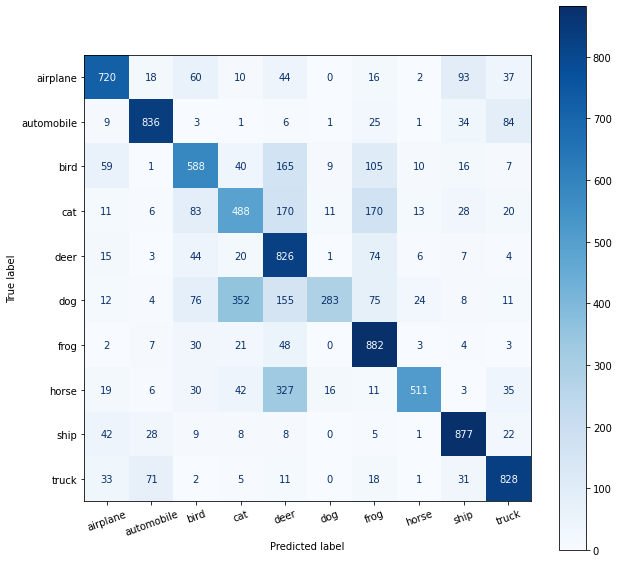
\includegraphics[width=.55\textwidth]{img/2_confusion_matrix}
  \caption{Matriz de confusión en validación para el modelo AlexNet tras 15 épocas.}
  \label{fig:2_confusion}
\end{figure}

Vemos que las clases que más se confunden son \textit{`dog'} por \textit{`cat'} y \textit{`horse'} por \textit{`deer'}. Esto tiene sentido, ya que en ambos casos se trata de animales de tamaño, color y características morfológicas parecidas, que dependiendo de la distancia, pose u oclusión pueden ser difíciles de diferenciar incluso para los seres humanos. También hay que tener en cuenta que es muy probable que las imágenes de las clases confundidas estén en un contexto parecido (ambientes domésticos para perros y gatos, y naturaleza para caballos y ciervos), dificultando aún más la clasificación.

\subsection*{Proyección t-SNE}

Podemos mostrar aquí también la proyección t-SNE de la representación de la capa final de la red, que se observa en la Figura \ref{fig:2_tsne}.

\begin{figure}[h!]
  \centering
  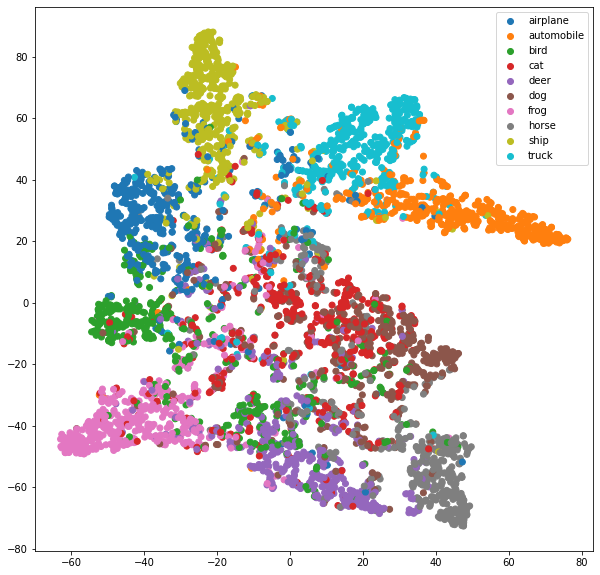
\includegraphics[width=.6\textwidth]{img/2_tsne_final}
  \caption{Proyección t-SNE en validación con la representación final de AlexNet.}
  \label{fig:2_tsne}
\end{figure}

En este caso no se observan clústers tan diferenciados y compactos como en MNIST. Sin embargo, vemos que las diferentes clases sí forman grupos más o menos separados, aunque con bastante dispersión y solapamiento. Por ejemplo, vemos que los clústers correspondientes a perros y gatos son los más dispersos y solapados, pues como dijimos antes estas clases son las dos que más se confunden. Algo parecido ocurre con las agrupaciones asociadas a pájaros y aviones o a camiones y coches, que también son confundidas con frecuencia por el modelo debido a las características de las imágenes: forma, tamaño, \textit{background} común, etc. Por todo esto, podemos pensar que la clasificación no será tan buena como en MNIST (de hecho, hemos comprobado que no lo es), pues el modelo no posee suficiente capacidad de discriminación.

Podríamos intentar aumentar el rendimiento del modelo con técnicas como \textit{data augmentation}, y también optimizando los hiperparámetros del modelo: el tamaño de \textit{batch}, el \textit{learning rate}, el propio optimizador, etc.
\newpage

\section{Transfer learning}

Esta última parte corresponde al notebook \verb|Transfer_Learning.ipynb|, donde experimentamos con técnicas de \textit{transfer learning} y \textit{finetuning} en el conjunto de datos externo \href{https://www.kaggle.com/pmigdal/alien-vs-predator-images}{Alien vs. Predator}, con un total de 894 imágenes RGB pertenecientes a dos clases. Empleamos cuatro enfoques distintos para intentar clasificar las imágenes:

\begin{enumerate}
  \item Entrenar un modelo desde cero (\textit{Scratch}).
  \item Utilizar una red preentrenada como extractor de características y clasificar con SVM lineal (\textit{Extractor + SVM}).
  \item Utilizar una red preentrenada con la última capa totalmente conectada adaptada a nuestro problema, y entrenarla unas pocas épocas más mediante finetuning (\textit{Finetune}).
  \item Igual que el anterior, pero haciendo \textit{data augmentation} (\textit{Finetune + augmentation}).
\end{enumerate}

\subsection*{Rendimiento de los modelos}

A continuación se muestra la máxima precisión conseguida con cada uno de los cuatro métodos:

\begin{table}[h!]
  \centering
  \begin{tabular}{c|cccc}
    & Scratch & Extractor + SVM & Finetune & Finetune + augmentation\\
    \hline
    Precisión máxima & 73.50\% & 90.50\% & 93.00\% & 95.50\%
  \end{tabular}
\end{table}

Vemos que hay una diferencia notable entre partir de un modelo sin entrenar y utilizar un modelo preentrenado, siendo esta última opción la que mejores resultados arroja.

\subsection*{Proyecciones t-SNE}

Finalmente, mostramos en la Figura \ref{fig:3_tsne} las proyecciones t-SNE obtenidas a partir de las representaciones finales de cada uno de los cuatro métodos. Junto a estas proyecciones mostramos también la frontera del hiperplano que ``mejor'' separa linealmente los datos proyectados (según un SVM lineal entrenado con ellos).

Observamos que en el caso de entrenamiento desde cero apenas se diferencian los clústers en la proyección, ya que están muy dispersos y solapados. En el resto de alternativas sí que vemos un patrón más claro en la nube de puntos, mejorando progresivamente y llegando a una separación casi perfecta con la última técnica de finetuning con data augmentation.

En cuanto al grado de separabilidad lineal, el método $1$ basado en entrenamiento desde cero presenta unos resultados que dejan bastante que desear, ya que la representación obtenida no es muy buena. Por otra parte, en el método $2$ de extracción de características la proyección tiene un grado aceptable de separabilidad lineal, aunque lejos de ser perfecto. El método $3$ mejora bastante la representación y la separabilidad, aunque aún comete algunos fallos. Finalmente, en el caso $4$ de finetuning con data augmentation obtenemos a la vez una separación de los datos proyectados y una precisión de clasificación en el espacio original casi perfectas, por lo que es claramente el modelo ganador. No obstante, para otros datasets o si dispusiéramos de menos datos de entrenamiento podría ser que algún otro de los enfoques fuera más adecuado.

\begin{figure}[h!]
     \centering
     \begin{subfigure}[b]{0.49\textwidth}
         \centering
         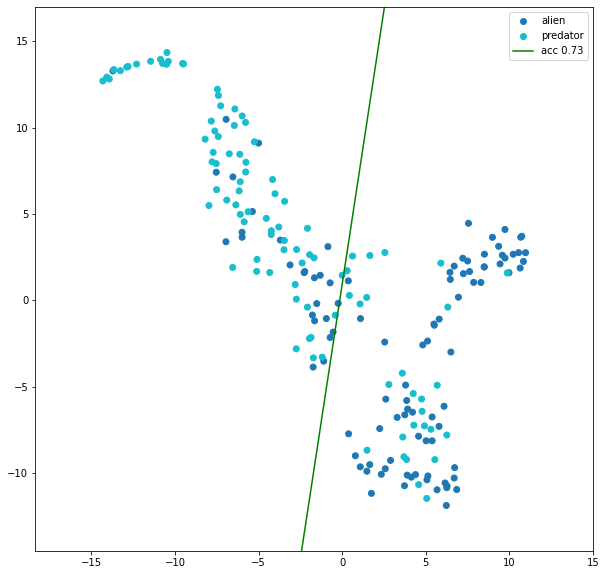
\includegraphics[width=\textwidth]{img/3_tsne_scratch}
         \caption{Scratch}
     \end{subfigure}
     \hfill
     \begin{subfigure}[b]{0.49\textwidth}
         \centering
         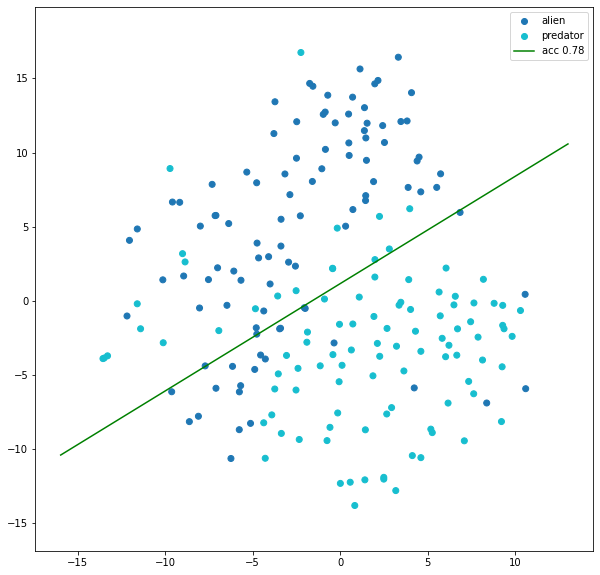
\includegraphics[width=\textwidth]{img/3_tsne_extractor}
         \caption{Extractor + SVM}
     \end{subfigure}
     \\
     \begin{subfigure}[b]{0.49\textwidth}
         \centering
         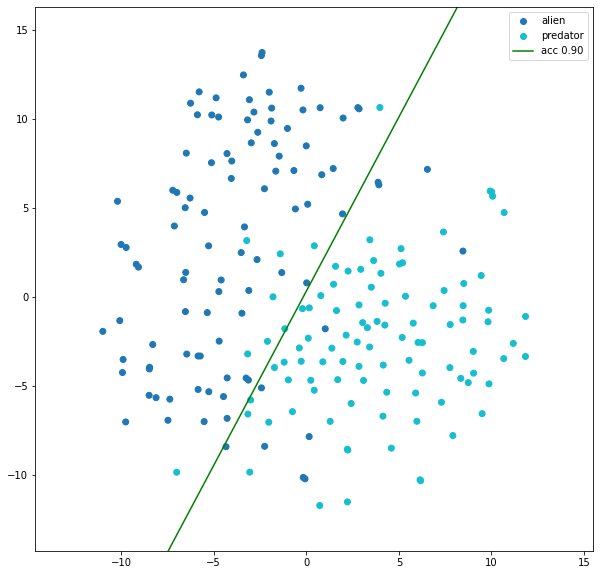
\includegraphics[width=\textwidth]{img/3_tsne_finetune}
         \caption{Finetune}
     \end{subfigure}
     \hfill
     \begin{subfigure}[b]{0.49\textwidth}
         \centering
         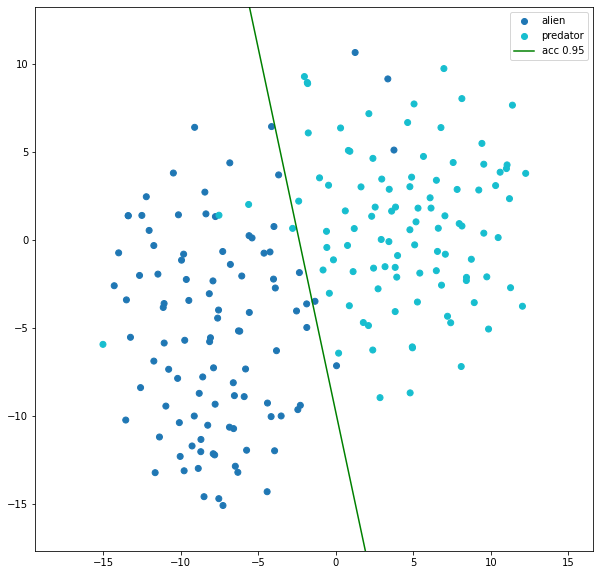
\includegraphics[width=\textwidth]{img/3_tsne_augmentation}
         \caption{Finetune + augmentation}
     \end{subfigure}
        \caption{Proyecciones t-SNE de las representaciones finales obtenidas en validación junto a los hiperplanos separadores para cada uno de los métodos probados.}
        \label{fig:3_tsne}
\end{figure}

\end{document}
